% TEMPLATE for Usenix papers, specifically to meet requirements of
%  USENIX '05
% originally a template for producing IEEE-format articles using LaTeX.
%   written by Matthew Ward, CS Department, Worcester Polytechnic Institute.
% adapted by David Beazley for his excellent SWIG paper in Proceedings,
%   Tcl 96
% turned into a smartass generic template by De Clarke, with thanks to
%   both the above pioneers
% use at your own risk.  Complaints to /dev/null.
% make it two column with no page numbering, default is 10 point

% Munged by Fred Douglis <douglis@research.att.com> 10/97 to separate
% the .sty file from the LaTeX source template, so that people can
% more easily include the .sty file into an existing document.  Also
% changed to more closely follow the style guidelines as represented
% by the Word sample file. 

% Note that since 2010, USENIX does not require endnotes. If you want
% foot of page notes, don't include the endnotes package in the 
% usepackage command, below.

%%%%%%%%%%%%%%%%%%%%%%%%%%%%%%%%%%%%%%%%%%%%%%%%%%%%%%%%%%%%%%%%%%%%%
\newcommand{\figref}[1]{Figure~\ref{#1}}
\newcommand{\secref}[1]{Section~\ref{#1}}
\newcommand{\tabref}[1]{Table~\ref{#1}}
\newcommand{\heading}[1]{\vspace{4pt}\noindent\textbf{#1}}
\newcommand{\noheading}[0]{\vspace{4pt}\noindent}
\newcommand{\program}[1]{\texttt{#1}}
\newcommand{\term}[1]{\texttt{#1}}
\newcommand{\captiontext}[1]{\textsf{\normalsize #1}}
\newcommand{\note}[2]{\textit{\textbf{\textcolor{#1}{#2}}}}
%%%%%%%%%%%%%%%%%%%%%%%%%%%%%%%%%%%%%%%%%%%%%%%%%%%%%%%%%%%%%%%%%%%%%


\documentclass[letterpaper,twocolumn,10pt]{article}
\usepackage{usenix,epsfig,endnotes}

\usepackage{multirow}
\usepackage{hhline}
\usepackage{color}
\usepackage{etoolbox}

\begin{document}

%don't want date printed
\date{}

%make title bold and 14 pt font (Latex default is non-bold, 16 pt)
\title{\Large \bf Towards Low-latency Geo-replicated Filesystem with Adaptive Remastering }

\author{
{\rm Peizhen Guo}\\
Yale University
\and
{\rm Bo Hu}\\
Yale University
}

\maketitle

% Use the following at camera-ready time to suppress page numbers.
% Comment it out when you first submit the paper for review.
\thispagestyle{empty}


%\subsection*{Abstract}
%Your Abstract Text Goes Here.  Just a few facts.
%Whet our appetites.

\section{Introduction}

\note{blue}{copied from proposal}

CalvinFS is a highly scalable distributed filesystem, which stores files metadata in a distributed database rather than in a single server. This design choice dramatically increases the scalability of the filesystem, and as well overcomes single-point failure of metadata server so that provides higher availability. However, such optimization incurs additional overhead on manipulating file metadata. Originally, modifying the metadata of a file only needs a single RPC call from the client to the metadata server, while now it needs a distributed transaction to achieve this goal.

Moreover, in order to fulfill stringent availability requirement, data are often replicated in geographically separated regions, to overcome the entire datacenter outage caused by natural disaster. In such scenario, the cross-region distributed transaction will result in unacceptably high latency. To be specific, in CalvinFS, the latency mainly stems from following two aspects: 1) the global ordering of all distributed transactions to maintain consistency between replicas; 2) Concurrency control when executing transactions, such as Two-phase Locking (2PL).
\section{Motivation}

\subsection{Background}
\subsubsection{Highly scalable geo-distributed file system}
Today, web-scale applications need to store and process a large amount of data. To provide the same responsive service to users all around the world, building a highly scalable geo-dsitributed file system is a must. However, previous geo-distributed file system utilized a fundamentally unscalable design for metadata layer management. Considering to reduce synchronization overhead because of replication or partition, they either use single-node or share-disk design to manage the metadata of the whole file system. The underling assumption is the file size in the system is large on average. Therefore, the metadata layer is small enough to be managed by a single-node or share-disk framework. 

However, that is not always the case, when there are large number of small files in the file system, there might not be enough space for a single node to manage these metadata. Moreover, the metadata management layer will obviously become a throughput bottleneck of the file system. To build a highly scalable geo-distributed file system, a highly scale metadata management system is a must.

\subsubsection{CalvinFS}
CalvinFS \cite{thomson2015calvinfs} is a metadata management system designed for the geo-distributed file system. Building on a distributed database system, Calvin, CalvinFS partitions and replicates metadata across a shared-nothing cluster of servers. It provides paxos-based strong consistency by posing a global deterministic transactions ordering. And also because of these global order, CalvinFS is a dead-lock system, which means it doesn't need a distributed commit protocol for distributed transactions. These two properties are largely improving the scalability as well as the throughput of the metadata management system when compared to traditional ones.

Unfortunately, high throughput and scalability come at a price. Compared to the single-node design, CalvinFS has a non-negligible latency. That is mainly coming from the Paxos-based consistency. It takes a server 2 RTTs from receiving the request to getting the global order of the transactions. And as the system itself is a geo-distributed, the average RTT between different replicas will be quite long, which makes the latency worse. Moreover, the latency will be even worse for the multi-file transactions, a server need to wait for collecting all the other related partitions' results to make real progress. The latency issue because of applying Calvin to metadata management system makes CalvinFS not a good choice.

\subsubsection{Master}
One key observation of this kind of geo-distributed file system is that a file or a directory is mostly accessed by a specific geo-replica. So, we can just let this specific replica take charge of the ordering of transactions involved with a range of files and directories, which we call "mastering" them in this paper. By letting each replica masters a partition of the metadata, we can determine the order of most transactions locally to reduce latency because of Paxos mechanism.  However, not all transactions are involved with files that mastered by only one replica. These multi-mastered transactions will make the latency and consistency become a problem. 

\subsection{Design Goals}
To reduce unnecessary latency, and as well not sacrificing strong consistency. We plan to replace time-consuming Paxos-like replication consensus protocol with a more lightweight protocol, which we call remastering protocol, to guarantee the total ordering without bringing inconsistency. Building on top of the master method, when receiving multi-mastered transactions, we first delay them to make all of the files in the transaction mastered by a single replica, and then process it as a new single-mastered transaction. In next section, we will introduce the design details of this protocol.

%Second, we plan to use machine learning algorithms to infer the access pattern of files and periodically adjust the master location based on such pattern, so as to make most transactions running locally, rather than cross geographic regions.
\section{System Design}

Our adaptive remastering mechanism is based on the CalvinFS~\cite{thomson2015calvinfs} system. CalvinFS leverages the features of Calvin, which avoids ordering operations when holding the locks to manage metadata storage for file system. However, low throughput stemmed from the long RTT between geo-distributed replicas requires us to adjust the system architecture to trim the cross-replica communication. In general, the key insight is that we assign each file with a local master replica to manage the read/write operations of this file, and transactions involved with only locally-mastered metadata will be serialized locally, without a cross-replica Paxos application to achieve global ordering. Hereby, we name our modified CalvinFS system as \name.

\subsection{System Components}
\name{} consists of following key components, \textsf{Scheduler}, \textsf{BlockLog}, \textsf{MetaStore}, \textsf{PaxosApp}, and \textsf{BlockStore}. As shown in Figure~\ref{fig:arch}, clients submit requests to \textsf{BlockLog}, which parses the transactions and distribute them to corresponding machines. Then it submits a batch of transactions to \textsf{PaxosApp} for ordering. \textsf{Scheduler} on each machine will fetch the output sequence of all transactions from the \textsf{PaxosApp} in local replica, and then call the \textsf{MetaStore} to execute the the transaction. In the following, we will delve into details about \textsf{Scheduler}, \textsf{BlockLog}, and \textsf{PaxosApp}, which carries the essential logic of CalvinFS.

\begin{figure*}[tp]
\centering
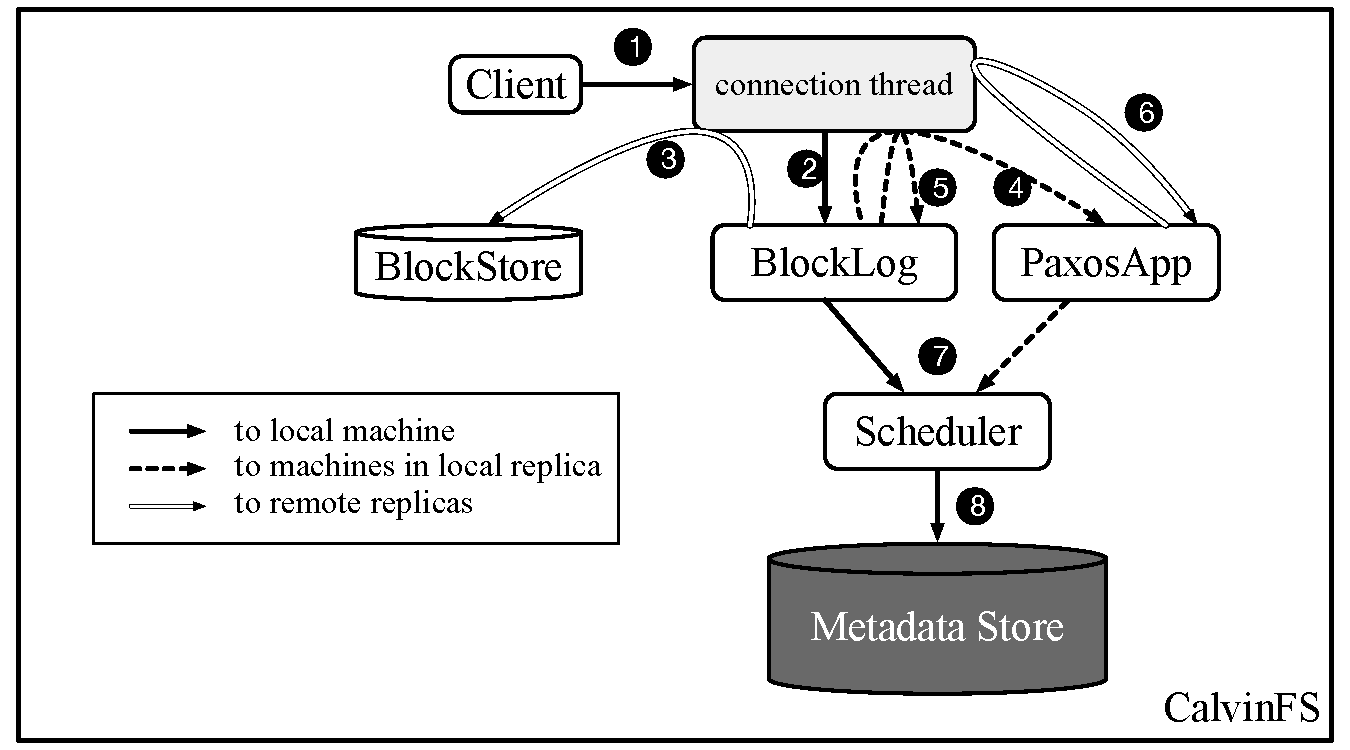
\includegraphics[width=1.8\columnwidth]{figures/arch}
\caption{Logical components of the CalvinFS and the interactions between them}
\label{fig:arch}
\end{figure*}

\heading{BlockLog} 

\noindent This module lies in the center of the \name{}. It interacts with clients, the scheduler, and the sequencer. Client will submit requests to the BlockLog application on the same machine. And, BlockLog will periodically pop all the pending requests in the queue, gather them into a batch, and send the batch to each replica for durability. After that, it will submit the batch ID to PaxosApp for a global sequence, because each machine concurrently receive and process requests from clients. BlockLog also interacts with the Scheduler module by exposing the interface where PaxosApp outputs the batch ID sequence to it.

\heading{Scheduler}

\noindent This module controls when a certain transaction will be executed by the Metastore, so as to guarantee the isolation property. It will first fetch the output sequence from the PaxosApp, and then tries to acquire locks from the readset and writeset of the transaction. Unlike common 2PL protocol, there is a deterministic order before processing the transaction, thus there is no need to release the lock when it is occupied by other ongoing transactions. After acquiring all locks, the Scheduler will call the MetaStore to execute the transaction asynchronously.

\heading{PaxosApp} 

\noindent In traditional CalvinFS, PaxosApp runs on only one machine in each replica, and all requests received by all the machines will be sent to the PaxosApp in their local replica. And, there is a simple Paxos protocol running among all participants from all replicas. To reduce the latency caused by cross-replica communication in Paxos protocol, metadata could be further partitioned into different parts, each of which is assigned to a local replica to manage. In this case, aside from serialize locally submitted requests, PaxosApp also has to coordinate with remote participants to realize the sequence of transactions belonging to other replicas. 




All aforementioned modules are located on each machine within each replica, and each module is registered as an application, running as an independent thread, and communicate with each other through a common communication thread (in each machine), which will further dispatch the messages to corresponding message handling thread to execute.

\subsection{Remaster Protocol}

\begin{figure}[tp]
\centering
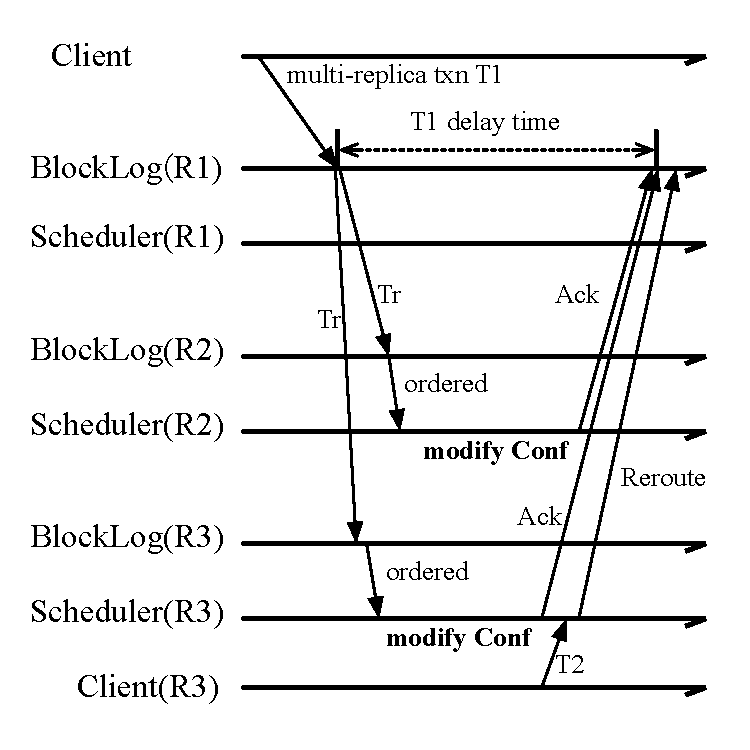
\includegraphics[width=\columnwidth]{figures/flow}
\caption{Explanation of how does Remaster protocol proceed when a distributed transaction T1 arrives}
\label{fig:flow}
\end{figure}

Previous transaction processing logic works well when the static partition of metadata perfectly matches the file access pattern where no distributed transaction appears. However, when there exists distributed transaction, realizing the order the transaction from other replicas will take at least 1 RTT, which means the local replica has to first acquires all locks and then wait at least 1 RTT before proceeding. This waiting time is large enough to impede the throughput of the system. On the other hand, it is extremely hard, if not impossible to achieve the perfect partitioning, not mention such partitioning could become unfit when time goes. Following this basic idea, we further extend static partitioning into an adaptive algorithm, which is called remaster, the master of each file is not statically decided but rather dynamically switched between replicas. In the following, we will introduce how we modify the logic of BlockLog and Scheduler so as to support remaster and as well the \name{} system.

Figure~\ref{fig:flow} illustrates the logic flow of the remaster protocol, and we will delve into details explaining how BlockLog and Scheduler modules work.

\subsubsection{BlockLog Logic}
In \name{}, each multi-replica transaction will incur an adjustment of the master replica assignment for those involved directory. Therefore, BlockLog will first check whether a transaction is multi-replica distributed transaction. If it is a multi-replica transaction, instead of creating a batch, BlockLog will pause this transaction in a specific waiting queue, and then it will create a special transaction, namely remastering transaction $T_r$, to all participating remote replicas, which will further modify their configuration when receiving such transaction, to note the change of the master for this directory.

We also add two additional message handling methods in BlockLog, reroute and remaster\_ack, respectively. When the remote replicas successfully change their configuration, they need to let the primary replica know it is legible to release waiting transaction to proceed as a local transaction in primary replica. Therefore, they send a remaster\_ack message to the BlockLog in primary replica, which will modify the configuration file of the primary replica and further selects those legible pending multi-replica transactions to create batch and begin running as a local transaction. Reroute method deals with the inconsistent views. When a transaction is falsely sent to a replica where it should not be executed, then once the Scheduler realize, it will call reroute method to resend the transaction to the right position.

\subsubsection{Scheduler Logic}
The Scheduler has to deal with the remaster transactions. When the remote replica's scheduler receives a batch of transaction, then for each transaction in it, it has to first verify whether it is a normal single-replica transaction, or it is a falsely sent transaction, or it is a remaster transaction which modify the configuration. The scheduler distinguishes the three cases by the keywords in transaction packet, including the original replica where it is received, and the remaster operation notifier. After realizing the status of the transaction, it will modify the configuration file if it is a remaster transaction; send a reroute RPC call to BlockLog if it is a falsely sent transaction; and acquire lock to execute the transaction if it is a normal single-replica transaction.








\section{Discussion}
In this section, we will discuss whether our protocol works under more tricky cases.
\subsection{Concurrent Remastering}
In previous section, we discussed the simplest case - a single remaster operation. Here, we will consider what if there are multiple concurrent remastering operations in the system. 
We have reroute mechanism to avoid falsely sent actions being ignored.

\subsection{Overlapping Remaster operation}
Only send remaster transaction once.


\subsection{Fail-over}
Can we bibi something in this part?? optional
feel heart lei, can not bibi anymore, just knee down to Abadi
\section{Implementation}
Summary
\subsection{BlockLopApp}

\subsection{Scheduler}


\section{Ongoing and future works}
Figuring out how to do the remastering operation itself is just the first step, we also need to figure out when and where to do it. This requires designing a \textbf{deadlock resolution strategy} to enable arbitrary direction of remastering,  a \textbf{profiling tools} to capture the file access pattern and a \textbf{learning algorithm} to discover underlying correlation between different files. We plan to keep track of this project and work with Kun to finish this part afterwards.

\subsection{Deadlock resolution}

\subsection{Profiling and learning}


\section{conclusion}





%%%%%%%%%%%%%%%%%%%%%%%%%%%%%%%%
\if 0
\section{Tentative Working Plan}

By communicating with Kun, we find that Kun has already done some works in this project. Instead of directly deploying remaster idea, Kun, instead, implemented a way to handle the ordering of distributed transaction requests. He proposed a tentative algorithm that each transaction will be broadcasted to all participating regions, and without running consensus protocol, each participating region independently decides their ordering and broadcast it. If they are inconsistent with each other, there will be deadlocks (cycles) in the transaction dependency graph. Therefore, the lightweight deadlock resolution algorithm is the main goal. Kun is currently working on this part. Hence, based on the current status, the overall plan of our final project consists of three stages, and each stage spans roughly two weeks.


For the first two weeks, we plan to get familiar with the code base of CalvinFS and catch up with the existing work Kun has done. And also, we’d like to work with Kun to figure out an elegant way to solve the deadlock problem. Kun said he has some tentative solution related to the deadlock problem, we will discuss about these solutions later with Kun in details. Hopefully, we can ramp up and move on to the remaster part in two weeks.


For the next two weeks, we plan to first work on enabling the remaster operation in the CalvinFS, One important point is to design a remastering protocol so as to guarantee strong consistency during remastering procedures. And also as the on-demand master migration is not supported by original CalvinFS, it will take some time for us to figure out how to enable this functionality. After finishing this part, we will move on to prepare for the in-class presentation and do some related evaluations.


For the last two weeks, we’d like to make it as a grace period. If some expected things happens, and we don’t manage to follow the time schedule, these two weeks is a good time for us to catch up with the schedule and finish the final report at last. 


\section{Evaluation}
We plan to evaluate our system, Super CalvinFS, in three aspects, deadlock resolution, adaptive remastering, and distributed transaction performance. The previous two aspects will be evaluated with micro-benchmark, to justify the correctness and performance of the two essential modules. For the last part, we plan to use standard benchmark, like TPC-C to test our performance under different settings. 

\indent \textbf{Deadlock resolution.} \,\,This session is related to the assessment of different deadlock resolution methods to find the most suitable one for the Super CalvinFS . 

\textbf{Remaster operation.} \,\,This part is mainly aimed at proving the correctness of remastering operation, as well as the response accuracy.

\textbf{Distributed transaction performance.} \,\,This session discusses the performance of the Super CalvinFS, including the throughput and latency, given different ratio of the distributed transactions within all transactions. We can get the maximum performance gain by using Super CalvinFS when there is no distributed transactions. And also, we can know the overhead of Super CalvinFS compared to CalvinFS when testing under the condition all of the transactions are distributed transactions~\cite{Einstein}.
\fi
%%%%%%%%%%%%%%%%%%%%%%%%%%%%%%%%


{\footnotesize \bibliographystyle{acm}
\bibliography{sample}}


%\theendnotes

\end{document}







